% Cancer is recognized as a major public health problem throughout the world
% and is the second most common cause of death in the United
% States~\cite{Siegel2016}. 

In recent years, chemotherapy based on targeted kinase inhibitors (TKIs) has
played an increasingly prominent role in the treatment of cancer. 
% The design
% of TKIs was inspired by modern genetic understanding of DNA, the cell cycle,
% and molecular signaling pathways. 
TKIs have been developed to selectively inhibit kinases involved in the
signaling pathways that control growth and proliferation, which often become
dysregulated in cancers. This targeting of specific cancers reduces the risk
of damage to healthy cells and increases treatment success. Currently, 
35 FDA-approved small molecule TKIs are in clinical use, and they represent a
significant fraction of the \$37 billion U.S. market for oncology
drugs~\cite{FDA, Zhao2014}. Imatinib, the first of these of drugs, is
partially credited for doubling survivorship rates in certain
cancers~\cite{Zhao2014, ACSreport}.

Unfortunately, the development of resistance to these drugs limits the amount
of time that patients can derive benefits from their treatment. Resistance to
therapeutics is responsible for more than 90\% of deaths in patients with
metastatic cancer~\cite{Longley2005}. While drug resistance can emerge via
multiple mechanisms, small changes to the chemical composition of the
therapeutic target (known as mutations) control treatment sensitivity and
drive drug resistance in many patients (see Fig.~\ref{fig:egfr}). In some
commonly targeted kinases such as Abl, these changes account for as many as
90\% of treatment failure~\cite{Shah2002}.

% \begin{figure}
%   \centering
%   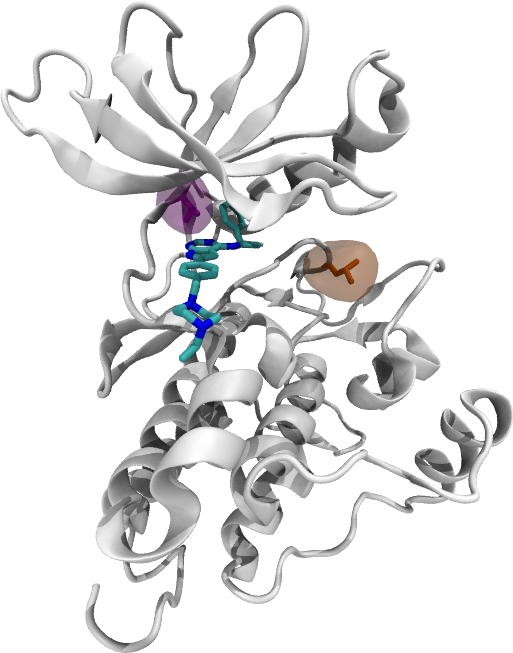
\includegraphics[width=0.60\columnwidth]{FIGURES/egfr.png}
%   \caption{Cartoon representation of the EGFR kinase bound to the inhibitor
%   AEE788 shown in chemical representation (based on PDB:2J6M). Two residues
%   implicated in modulating drug efficacy are highlights; in pink T790 and in
%   orange L858. Mutations to either of these residues significantly alter the
%   sensitivity to TKIs.}\label{fig:egfr}
% \end{figure}

There are two major strategies for countering the threat to treatment
efficacy posed by resistance: tailoring the drug regimen received by a
patient according to the mutations present in their particular cancer, and
developing more advanced % second- or third-line
therapies that retain potency for known resistance mutations. In both cases,
future developments require insight into the molecular changes produced by
mutations, as well as ways to predict their impact on drug binding on a
timescale much shorter than is typically experimentally feasible. This
represents a grand challenge for computational approaches.

The rapidly decreasing cost of next-generation sequencing has led many cancer
centers to begin deep sequencing of patient tumors to identify the genetic
alterations driving individual cancers. The ultimate goal is to make
individualized therapeutic decisions based upon these data---an approach
termed \textit{precision cancer therapy}. While several common (recurrent)
mutations have been cataloged for their ability to induce resistance or for
their susceptibility to particular kinase inhibitors, the vast majority of
clinically observed mutations are rare. Essentially, this ensures that it
will be impossible to make therapeutic decisions about the majority of
individual patient tumors by using catalog-building alone.

Fortunately, concurrent improvements in computational power and algorithm
design are enabling the use of molecular simulations to reliably quantify
differences in binding strength. This provides the opportunity to use advances
in molecular simulations to supplement existing inductive decision support
systems with deductive predictive modeling and drug ranking~\cite{Marias2011,
Sloot2009}. Where existing systems based on statistical inference are
inherently limited in their range of applicability by the existence of data
from previous similar cases, the addition of modeling allows evidence based
decision making even in the absence of direct past experience.

% This provides the opportunity to use automated simulation workflows to
% supplement existing inductive (`Baconian') decision support systems with
% deductive (`Popperian') predictive modeling and drug
% ranking~\cite{Marias2011, Sloot2009}. Where existing systems based on
% statistical inference are inherently limited in their range of applicability
% by the existence of data from previous similar cases, the addition of
% modeling allows evidence based decision making even in the absence of direct
% past experience.

The same molecular simulation technologies that can be employed to
investigate the origins of drug resistance can also be used to design new
therapeutics. Creating simulation protocols which 
% meet the varying demands of different applications and 
have well defined uncertainty and produce
% (such as the rapid turn around times needed for clinical decision support)
% whilst obtaining
statistically meaningful results represents a significant
computational challenge. Furthermore, it is highly likely that differences
among % the varied 
investigated systems % which might be investigated 
will demand different protocols
as studies progress. For example, % in 
drug design programmes % it is usual to need 
often require the rapid screening of thousands of candidate compounds to filter
out the worst binders before using more sensitive methods 
% are required when refining 
to refine the structure. Not all changes induced in protein shape or
behavior are local to the drug binding site and, in some cases, simulation
protocols will need to adjust to account for complex interactions between
drugs and their targets within individual studies.

Recent work that used molecular simulations to provide input to machine
learning models~\cite{Ash2017} required simulations of 87 compounds even if
they were designed merely to distinguish the highly active from weak
inhibitors of the ERK2 kinase. If we wish to build on such studies to help
inform later stages of the drug discovery pipeline, in which much more subtle
alterations are involved, it is likely a much larger number of simulations
will be required. This is before we begin to consider the influence of
mutations or the selectivity of drugs to the more than 500 different
genes in the human kinome~\cite{Li2016}.

For molecular simulations to make the necessary impact, the dual challenge of
scale (thousands of concurrent multi-stage pipelines) and sophistication
(adaptive selection of binding affinity protocols based upon statistical
errors and uncertainty) will need to be tackled. Tools that facilitate the
scalable and automated computation of varied binding free energy calculations
on high-performance computing resources are necessary. To achieve that goal,
we introduce the High-throughput Binding Affinity Calculator~(HTBAC). HTBAC
translates recent advances in workflow system building blocks to the
application of rapid and accurate calculation of  binding affinities. We
demonstrate how HTBAC scales almost perfectly to hundreds of concurrent
pipelines of binding affinity calculations on a leadership class machine. This
permits the rapid time-to- solution that is essentially invariant of the size
of candidate ligands as well as the type and number of protocols concurrently
employed.

In the next Section, we provide details of ensemble molecular dynamics
approach and its advantages (i.e., greater accuracy) over single trajectory
approach. We also introduce the ESMACS and related protocols to compute
binding affinities using ensemble based approaches. In Section 3, we discuss
the computational challenges associated with the scalable execution of
multiple, and possibly concurrently executing protocols. Section 4 introduces
RADICAL-Cybertools -- a suite of building blocks to address the challenges
outlined in Section 3. In Section 5 we introduce HTBAC and describe how it
uses RADICAL-Cybertools to support the needs of binding affinity calculations
at extreme scales. Experiments to characterize the performance and scalability
of HTBAC on the Blue Waters supercomputer are discussed in Section 6. We
conclude with a discussion of the impact of HTBAC, implication for binding
affinity calculations and near-term future work.

%\jhanote{Is there a need for differentiation across these thousands of
%candiate compounds, or must they by design be treated and subject to the
%same protocols?}

%\jhanote{SJ to introduce extreme scale/exascale systems and provide stronger
%motivation for HTBAC}

% The strength of drug binding is determined by a thermodynamic property
% known as the binding free energy (or binding affinity). One promising
% technology for estimating binding free energies and the influence of
% protein composition on them is molecular dynamics (MD). In order to study
% the influence of mutations on drug binding atomistically detailed models of
% the drug and target protein can be used as the starting point for MD
% simulations. The chemistry of the system is encoded in what is known as a
% potential. \cite{Karplus2002} In the parameterization of the models each
% atom is assigned a mass and a charge, with the chemical bonds between them
% modelled as springs with varying stiffness. Using Newtonian mechanics the
% dynamics of the protein and drug can be tracked and using the principles of
% statistical mechanics estimates of thermodynamic properties obtained from
% simulations of single particles. The potentials used in the simulations are
% completely under the control of the user which allows the user to
% manipulate the system in ways which would not be possible in experiments. A
% particularly powerful example of this is so called `alchemical' simulations
% in which the potential used in the simulation changes from that
% representing one system to another during execution — allowing the
% calculation of free energy differences between the two systems (such as
% those induced by a protein mutation).

% MD simulations can reveal how interactions change as a result of mutations,
% and account for the molecular basis of drug efficacy. This understanding
% can form the basis for structure based drug design as well as helping to
% target existing therapies based on protein composition. Major challenges
% however exist in correctly capturing the system behaviour. Not only is it
% necessary that the approximations made in the potential are accurate enough
% representations of the real system chemistry but sufficient sampling of
% phase space is also required.

% %something about sampling techniques%

% In order for MD simulations to be used as part of clinical decision support
% systems it is necessary that results can be obtained in a timely fashion.
% Typically interventions are made on a timescale of a few days or at most a
% week. This need for rapid turn around times places additional demands on
% simulation protocols which need to be optimised to gain results within a
% short turn around time.

% Further to the scientific and practical considerations outlined above, in
% order for simulations to provide actionable predictions it is vital that
% robust and reliable uncertainty estimates are provided alongside all
% quantitative results. We have developed a number of free energy calculation
% protocols based on the use of ensemble molecular dynamics simulations with
% the aim of meeting these requirements \cite{Sadiq2008, Sadiq2010,
% Wan2017brd4, Wan2017trk}. Basing these computations on the direct
% calculation of ensemble averages facilitates the determination of
% statistically meaningful results along with complete control of errors. The
% consequence of the use of the ensemble approach is the need to automate the
% simulation, analysis and data transfer of a large number of simulations.
% This computational pattern necessitates the use of middleware that provides
% reliable coordination and distribution mechanisms with low performance
% overheads.